\chapter{Conclusions and future work}

\ifpdf
    \graphicspath{{Chapter7/figs/raster/}{Chapter7/figs/pdf/}{Chapter7/figs/}}
\else
    \graphicspath{{Chapter7/figs/vector/}{Chapter7/figs/}}
\fi
\section{Introduction}
The Multi-scale modelling of granular flows 
involves simulating the granular 
materials in discrete and continuum scales. In 
the present study, a C++ code 
has been developed to model the granular 
materials as discrete-elements using 
the Discrete Element Method technique. The 
Material Point Method code, 
developed in 
the University of Cambridge, has been adopted to 
study the flow of granular 
materials as a continuum. Multi-scale analyses 
of the collapse of the granular columns with 
different aspect ratios were 
performed using continuum and particle-scale 
approaches. In the present study, 
the solid-fluid interactions in the Discrete 
Element approach is modelled by 
coupling the Lattice Boltzmann Method, a 
Newtonian fluid solver, with the 
Discrete Element Method technique. This chapter 
presents an overview of the 
future 
research along with the proposed research 
schedule. This chapter also presents 
an outline of the final thesis and the proposed 
papers based on this research 
work. 


\section{Recommendations for future research}
This research work involves the following stages: 
(1) understanding the limits 
of the continuum and the discrete-element 
approaches in modelling the granular 
flow, and investigating the influence of various 
microscopic parameters on the 
macroscopic flow behaviour, (2) understanding the 
differences in the mechanism 
of the granular flows in dry and submerged 
conditions, and (3) Modelling the 
granular flow behaviour using the $\mu(I)$ 
rheology for dry and submerged flow 
conditions.

\subsection{Multi-scale simulations of granular 
flows}
The continuum and discrete-element simulations of 
the dry and the submerged 
granular flows will be performed to understand 
the differences in their flow 
mechanism. Multi-scale analyses of granular flows 
enable us to understand the 
limitations of the continuum approach in 
modelling large deformation granular 
flow problems, and help us to identify the 
micro-scale parameters responsible 
for the complex macroscopic behaviour. 
Multi-scale modelling of the collapse of 
a granular columns on a horizontal surface have 
been performed. Continuum 
simulations accurately predict the granular flow 
behaviour for columns with 
smaller aspect ratios, however they fail to 
capture the dynamics of the flow 
for columns with larger aspect ratios. 

In order to understand the difference in the flow 
dynamics with increasing 
aspect ratios, further analyses will be performed 
to study the mechanism of 
energy dissipation in the particle scale, i.e. 
the evolution of kinetic energy 
and potential energy with time. A simple 
mathematical relationship based on the 
initial potential energy of the grains lying 
above the failure surface is being 
developed to describe the flow dynamics of the 
granular column collapse problem 
with different aspect ratios. The relationship 
will enable us to understand the 
variation in the flow dynamics in the continuum 
and the particle-scale. The 
continuum description of granular column collapse 
showed non-physical behaviour 
near the foot of the column, further analyses 
will be carried out to understand 
the effect of interface properties on the run-out 
distance. Further details on 
the continuum modelling of granular flow are 
presented in the next section. 
Micro-scale parameters influencing the flow 
dynamics will be identified and the 
influence of these parameters on the deposit 
morphology will be investigated. 
Multi-scale analysis of large deformation flow 
problem such as flow of dry 
granular materials down an inclined flume will be 
performed. This analysis will 
provide an insight on the limits of the continuum 
approach in modelling large 
deformation problems, which involve large 
shear-rates. The results from the 
analysis will be compared with the experimental 
results 
of~\citet{Denlinger2001} on miniature flume 
experiments. The influence of 
parameters, such as particle size, density, 
packing and dilatancy, on the flow 
dynamics will be explored. These studies will be 
useful in describing the 
granular flow behaviour using the $\mu(I)$ 
rheology.

In order to understand the differences in the 
mechanism between the dry and the 
submerged granular flows, multi-scale analysis of 
granular flows in fluid will 
be performed. In particle-scale approach, the 
Discrete Element Method technique 
coupled with Lattice Boltzmann approach will be 
adopted to study the collapse 
of granular columns in fluids. Dynamic 
fluid-coupling in the Material Point 
Method will be developed to study the behaviour 
of granular flows in fluids. 
The numerical simulations will be verified with 
the experimental results 
of~\cite{Cassar2005} on immersed granular flows. 
The effect of packing density 
of granular material, frictional parameters and 
the viscosity of the fluid on 
the flow dynamics and the phase-transition 
behaviour will also be investigated. 
The influence of the fluid viscosity on the flow 
behaviour will also be 
investigated. The variation in the flow dynamic 
and the deposit morphology for 
dry and submerged granular flows will also be 
analysed. The parameters that 
cause a change in the flow dynamic between the 
dry and the submerged flow 
conditions will be used in extending the $\mu(I)$ 
rheology for submerged 
granular flows. 


\subsection{Developments in Material Point Method}
The present MPM code is capable of solving the 
granular flow problems using the 
Mohr-Coulomb constitutive model. It is also 
capable of solving seepage problems 
with static fluid-solid interface. In the present 
study, the Material Point 
Method will be extended to solve 3D problems and 
it will be implemented into a 
standard framework, similar to the Finite Element 
framework developed in the 
University of Cambridge. Constitutive models such 
as Nor-Sand and $\mu(I)$ 
rheology will be implemented to model the dense 
granular flows. Modified 
Nor-Sand constitutive model~\citep{Robert2010} 
implemented in the present study 
will be validated by performing element testing 
and the results will be 
verified with the results 
of~\citet{jefferies2005}. The current MPM code is 
capable of simulating only small deformation 
problems, however special 
attention is required in modelling large 
deformation problems, especially those 
involving two-phase systems. Objective stress 
rate such as Jaumann stress rate 
has been implemented to study large deformation 
problems. The dynamic 
re-meshing technique~\citep{shin2010a} will be 
implemented to efficiently solve 
large deformation problems. The dynamic meshing 
approach is useful for problems 
involving motion of a finite size body in 
unbounded domains, in which the 
extent of material run-out and the deformation is 
unknown a priori. The 
approach involves searching for cells that only 
contain material points, 
thereby avoiding unnecessary storage and 
computation. 

The present fluid coupling algorithm in the MPM 
involves only static 
boundaries, and conserves the equation of 
momentum for fluid particles by 
introducing additional particles in a cell, when 
the number of particles 
decreases. A dynamic solid-fluid interface 
modelling in the Material Point 
Method will be developed. The approach involves 
the following steps: 
identification of the soil particles along the 
boundary of the current soil 
domain, obtaining the nodal numbers for the edges 
of each soil particle and 
definition of a new boundary (see 
Figure~\ref{fig:MPMFluidB}). The shape of the 
boundary is approximated by equivalent 
rectangular grids, similar to the 
coupling technique adopted in the 
discrete-element approach. The procedure is 
repeated until the entire boundary is defined. 
This process is repeated for 
each time step to simulate the dynamic boundary 
behaviour which is common in 
the case of granular flows in a fluid. 

The MPM code will be extended to include the 
phase-transition behaviour in a 
continuum domain for partially fluidized granular 
flows~\citep{Aranson2002, 
Aranson2001, Volfson2003}. The theory is based on 
the hydrodynamics of the 
flow, coupled with an order parameter equation, 
which describes the transition 
between the flowing and the static components of 
the granular system. The order 
parameter is defined as a fraction of static 
contacts among all contacts 
between particles. The shear stresses in a 
partially fluidized granular matter 
is assumed to have two components: the dynamic 
part that is proportional to the 
shear strain rate and the strain-independent or 
the static part. The ratio of 
these two parts is a function of the order 
parameter. The relative magnitude of 
the static shear stress is controlled by the 
order parameter which varies from 
0 in the liquid phase to 1 in the solid phase.

\begin{figure}[htbp]
\centering
\includegraphics[width=0.95\textwidth]{MPMFluidB}
\caption{Identification of dynamic solid-fluid 
boundary}
\label{fig:MPMFluidB}
\end{figure}

\subsection{The I rheology}

The $\mu(I)$ rheology is capable of describing 
the behaviour of dense granular 
flows. However, it considers the yield strength 
as an adjustable rheological 
property, which contradicts the basic 
understanding that the
strength evolves as the debris-flow motion 
progresses. Also, the $\mu(I)$ 
rheology uses the Mohr-Coulomb constitutive model 
to describe the yielding of 
granular materials. In the present study, the 
evolution of soil strength 
with time will be considered using models based 
on critical state framework. 
Nor-Sand constitutive model will be implemented 
in the present study to 
describe the plastic flow of granular materials. 
The $\mu(I)$ rheology will be 
extended to describe the behaviour of granular 
flows in fluids. In the case of 
dense granular flows, the parameter \textit{I} is 
described as the ratio 
between the time taken for a particle to fall 
into the hole, $t_{micro}$, and 
the meantime, $t_{mean}$, which is inversely 
related to the shear rate. If the 
velocity of the ambient fluid is low, then the 
time taken by the particle to 
fall into a hole, is then controlled by the 
viscosity of the ambient 
fluid~\citep{Pouliquen2005}. The $\mu(I)$ 
rheology will be modified to include 
the effect of fluid viscosity to model granular 
flows in fluids based on the 
parameters identified to control the flow 
dynamics.
\subsection{Homogenization of granular flows}
Granular materials are composed of grains in 
contact, and are therefore 
discontinuous and heterogeneous. The macroscopic 
material properties of these 
materials are liked to the fabric of the medium. 
It is interesting to define 
the behaviour of granular materials at the 
macroscopic scale from 
characteristics defined at the local scale. This 
approach has been widely 
developed for heterogeneous continuum and is 
known as the homogenization 
method. This kind of approach is different from 
the phenomenological one, in 
which the constitutive model is derived from the 
general laws of 
thermodynamics. These phenomenological models 
introduce some material 
parameters whose values are obtained from the 
simulations performed on 
representative volume element. The main objective 
of the homogenization method 
is to obtain a constitutive relation at the scale 
of a representative volume 
element, based the information on the material 
behaviour at the micro-scale and 
the micro-structure. For granular media, the 
micro-scale is generally the grain 
scale. The scale of the representative volume 
element is of several orders of 
magnitude higher. The homogenization process is 
based on three relations, a 
localization operator, a local constitutive law 
and an averaging operator, see 
Chapter 6. An intrinsic difficulty in the case of 
granular materials arise from 
the fact that the variables at the micro-scale 
and the macro-scale are of 
different nature. At the micro-scale the material 
behaviour is described using 
vectorial variables such as contact forces, grain 
displacement and grain 
rotation, where as the macroscopic behaviour law 
uses tensorial variables 
(stress tensor, strain tensor). The micro-polar 
plasticity constitutive 
formulation~\citep{Suiker2001} that is directly 
related to micro-scale 
properties, such as contact stiffness, particle 
density, particle radius and 
its micro-structure will be extended to large 
scale deformation problems which 
involves loss or gain of contacts between grains. 
Discrete Element Method 
simulations provide useful insight on the role of 
contact forces at 
micro-scale. The macroscopic stress is related to 
microscopic contact forces 
using the virtual work theorem. The microscopic 
kinematic variables usually 
considered are the displacement of the centre of 
mass of the particle and the 
ration of the particle. The local phenomena 
occurring at the micro-scale during 
the deformation of granular material are complex. 
Different approaches have 
been proposed in the literature to establish the 
link between particle-level 
displacements and macro-scale deformations. The 
micro-behaviour is converted 
into a macroscopic model through the conservation 
of internal work. The local 
constitutive law gives the value of contact 
forces and the average over the 
sample provides the value of the stress tensor. 

\subsection{Slope subjected to impact}
This work may be pursued along two directions: 1) experimental 
realization of a similar setup with different modes of energy injection and 
2) investigating the effect of various particle shapes or the presence of an 
ambient fluid. Although numerical simulations are generally reliable 
with realistic results found in the past studies of steady flows, we believe 
that the transients are more sensitive situations than steady states and the  
experiments are necessary for checking the validation of the results suggested 
by the simulations. Provided a convenient method is used for supplying kinetic 
energy homogeneously into a pile, our configuration is also interesting for 
the investigation of the behavior of a pile immersed in a viscous 
fluid.